\documentclass[a4paper, 12pt, titlepage]{article}

% osnovni paketi za jezik in kodiranje znakov
\usepackage[slovene]{babel} 
\usepackage[utf8]{inputenc}
\usepackage[T1]{fontenc}
\usepackage{lmodern}

% dodatni paketi
\usepackage{amsmath, amssymb, amsthm}
\usepackage[font=small, center]{caption}
\usepackage[hidelinks]{hyperref}
\usepackage{graphicx}
\usepackage{wrapfig}
\usepackage{float}     
\usepackage{geometry}
\geometry{tmargin=1.5in, textwidth=6.5in}
\usepackage[table]{xcolor} % http://ctan.org/pkg/xcolor
\usepackage{biblatex}
\addbibresource{literatura.bib}

% priprava strani
\pagestyle{headings}

\begin{document}

\begin{titlepage}
    \begin{center}
        \large
        Fakulteta za matematiko in fiziko\\
        \vspace{8cm}
        \Huge
        \textbf{NAKUP STANOVANJA} \\
        \vspace{7cm}
        \large
        Terezija Krečič\\
        Pedagoška matematika\\
        \vspace{1cm}
        Mentor: Petar Pavešić\\
        \vspace{0.5cm}
        Ljubljana\\
        16. april 2022
    \end{center}
\end{titlepage}

\tableofcontents
\newpage

%%%%%%%%%%%%%%%%%%%%%%%%%%%%%%%%%%%%%%%%%%%%%%
\section{Uvod}

Kaj ima nakup stanovanja skupnega z matematiko? Prva misel je lahko: ``Logično, saj imamo opravka z velikimi številkami, ki izginejo iz našega bančnega računa.'' Seveda to ni napačno. Vendar je tu še nekaj, s čimer se je po večini drugo polovico prejšnjega stoletja ukvarjalo že veliko znanih matematikov.

V nadaljevanju boste spoznali najbolj osnoven način reševanja svetovno znanega problema, znanega pod imenom \emph{``the secretary problem''}, ki se ukvarja z iskanjem najboljšega načina za izbor najboljšega elementa iz ponujene ponudbe. Izbira je omejena s pogojem, da si ogledujemo po en element naenkrat in se moramo na licu mesta odločiti, ali ga izberemo ali ne. To precej oteži reševanje, vendar nam prav zato vzbudi zanimanje in motivacijo, da bi ta izziv rešili, na koncu pa smo lahko nagrajeni z zadovoljstvom nad rešeno nalogo. Lahko se zgodi tudi, da nam to ni dovolj in se nam porodi še kakšno podobno vprašanje, dodaten ali pa milejši pogoj, in se potem sami lotimo nadaljnega reševanja.

Matematika dandanes veliko ljudem povzroča težave. Vse se začne že v šoli. Snov se kopiči, domače naloge so nerazumljive, učitelji nervozni \ldots Rado se zgodi, da so to glavni razlogi, da nekdo zasovraži matematiko in nič na svetu ga ne more prepričati, da je matematika lepa in lahko velikokrat olajša stvari. Primer: kmet ima 100 metrov ograje in bi z njo rad ogradil čim večji pašnik za koze. Če je kaj odnesel iz srednje šole, lahko na hitro zapiše tri vrstice računa z odvajanjem in dobi, da se mu najbolje splača očrtati kvadrat s stranico 25 metrov. Lahko mu pomagajo tudi izkušnje. Če pa nima ne enega ne drugega, kdo ve, za koliko trave bi prikrajšal svoje koze.

Ta seminar se prav tako ukvarja s praktičnim problemom iz vsakdanjega življenja. V ozadju se ne skriva skoraj nič matematične teorije, ki je ne bi spoznali na povprečni slovenski gimnaziji, zato je vsebina primerna tudi za vse nadebudne dijake, ki jim je matematika blizu. Če se ne počutite tako kompetentni, brez skrbi. Besedilo je zapisano tako, da je lahko razumljivo komurkoli, ki ima vsaj nekaj osnovnega znanja iz verjetnosti. Seveda pa je najbolj zanimiv rezultat in verjamem, da boste ta način reševanja kdaj tudi sami uporabili v praksi.

\newpage
%%%%%%%%%%%%%%%%%%%%%%%%%%%%%%%%%%%%%%%%%%%%%%
\section{Formulacija problema}

Zamislimo si, da si kupujemo novo hišo ali stanovanje. V časopisih in na internetu smo poiskali nek izbor stanovanj, vendar nas edina slika in kratek opis vsakega stanovanja seveda ne prepriča. Preden kupimo novo stanovanje, si ga želimo \emph{vsakega posebej} dobro ogledati. Naša želja je, da bi si kupili \emph{najboljše} stanovanje iz izbora (naivno predpodstavimo, da tu denar ni ovira), zato se kmalu podamo na ogled.

Najenostavnejši in tudi najefektivnejši način, s katerim bi poiskali najboljše stanovanje, je, da si ogledamo vsa stanovanja iz ponudbe in se na koncu odločimo za najboljšega. Žal se v realnem svetu človek na to težko zanese. Ogledi in ocenjevanje stanovanj vzamejo veliko časa, pa tudi samih ponudb stanovanj imamo lepo število. Kdo ve, ali bo stanovanje, ki smo si ga ogledali mesec nazaj in nam je bilo precej všeč, še na voljo? Zato si postavimo pravilo:

\begin{quote}
Ogledujemo si po eno stanovanje naenkrat. \textbf{Po vsakem ogledu se moramo odločiti, ali bomo to stanovanje kupili ali ne.} Pred odločitvijo si ne moremo ogledati naslednjih stanovanj in ne vemo, kakšna so. Če se odločimo to stanovanje kupiti, se tu z ogledom ustavimo, če pa se odločimo, da si ogledamo naslednje stanovanje, ponudbo trenutnega stanovanja izgubimo. Torej \textbf{ni poti nazaj.}
\end{quote}
\label{pogoj_za_nakup}

Zaradi tega pogoja sedaj pridemo do glavnega vprašanja -- kako izbirati, da dobimo najboljše stanovanje iz ponudbe? Pogoj nas precej omeji in jasno je, da so se nam s tem precej zmanjšale možnosti uspeha. Posledica je tudi, da če se do zadnjega stanovanja ne odločimo za nakup, moramo kupiti zadnje stanovanje, ne glede na njegovo stanje. Izkaže pa se, da so verjetnosti, da uspemo kupiti najboljše stanovanje, različne glede na način izbiranja. Sedaj smo prišli do bistva tega problema:

\begin{center}
\large
\texttt{Iščemo način, ki maksimizira verjetnost, da je izbrano stanovanje res najboljše od vseh}.
\end{center}

\subsection{Različice in drugi primeri}

Ta problem, ki se v tem seminarju imenuje \emph{nakup stanovanja}, je po svetu bolj znan kot \emph{``the secretary problem\footnote{problem tajnika, op. prev.}''}. Ima še veliko drugih imen, ki pa nimajo uradnega slovenskega prevoda: \emph{the marriage problem, the sultan's dowry problem, the fussy suitor problem, the googol game, the best choice problem}\footnote{poročni problem, problem sultanove dote, problem izbirčnega snubca, guglov problem (1 gugol je število, ki ji sledi sto ničel, torej $10^{100}$), problem najboljše izbire, op. prev.} \ldots

Poglejmo si nekaj primerov iz vsakdanjega življenja, iz katerih izhajajo tudi nekatera od naštetih imen:

\begin{itemize}
    \item Kot šef podjetja iščemo novega tajnika, na razpisano mesto pa se je prijavilo več kandidatov. Radi bi izbrali najboljšega, zato vsakega posebej intervjujamo. Takoj po intervjuju se moramo odločiti, ali bomo kandidata zaposlili ali ne. V primeru zaposlitve se ostale kandidate razpusti, ne da bi jih vse spoznali, v nasprotnem primeru pa si bo kandidat poiskal delo drugje in se ne bo več vrnil nazaj.
    \item Sedaj smo mi v vlogi iskalca službe in imamo neko ponudbo različnih del. Na intervjuju za eno od teh mest nam ponudijo delo. Ga sprejmemo ali iščemo dalje? Kaj pa, če nam nikoli več ne ponudijo tako dobrih delovnih pogojev?
    \item V življenju lahko gremo skozi več partnerskih zvez, vendar bi se enkrat radi ustalili. Sredi ene zveze se vprašamo: ``Ali je to res to? Ali se mi splača tvegati, pretrgati zvezo in upati, da dobim še kaj boljšega?''
    \item Sultan si izmed vrste princes izbira novo ženo za svoj harem, izbira pa jih glede na višino dote, ki bi jo prinesla v njegovo palačo. Kako naj se odloča, če si ogleduje po eno princeso naenkrat in odslovljenih princes ne more dobiti nazaj, saj se poročijo drugam?
    \item Prodajamo hišo, avto ali kako drugo dragoceno stvar. Prejemamo veliko različnih ponudb, saj dovolimo barantanje, vendar se vsakič vprašamo, ali je trenutna ponudba dovolj dobra ali lahko upamo na kaj več.
    \item Nakupujemo v trgovini in si ogledujemo nek izdelek. Ali ga naj kupimo danes ali lahko upamo na akcijo naslednji teden?
    \item Guglova igra (angl. ``The Googol Game''): vsak od n ljud na svoj listek zapiše eno število med 1 in $10^{100}$ (en gugol) ter ga odvrže v skupno košaro. Prostovoljec si želi izbrati čim večji listek iz košare. Jemlje po en listek naenkrat in vsakič se mora odločiti, ali se bo ustavil ali naj žreba dalje. Igra ima več različic.
\end{itemize}

Ostalih primerov je še veliko. Vsem je skupno, da se pri izbiri najboljšega od nekega nabora kandidatov upošteva podoben pogoj kot na strani~\pageref{pogoj_za_nakup}. Pri vseh pa obstaja tveganje -- kaj pa, če nihče od naslednjih kandidatov ne bo boljši od trenutnega? V tem primeru končamo z zadnjim kandidatom, ne glede na njegovo kakovost in vaše zadovoljstvo.

\subsection{Matematična formulacija}
Problem lahko prevedemo v matematiko s pomočjo naključnih zaporedij. Imamo $N$ stanovanj. Če bi si jih lahko brez škode vsa ogledali, bi jih lahko ocenili od 1 (najslabše stanovanje) do $N$ (najboljše stanovanje). Ker je vrstni red stanovanj naključen, imamo v bistvu pred seboj neko permutacijo iz množice $S_{N}$.

Tako kot si stanovanja ogledujemo po vrsti, tudi tu po zaporedju potujemo od začetka proti koncu, recimo od leve proti desni. Na vsakem koraku se odločamo, ali bi lahko bilo trenutno število največje v zaporedju. Če ga izberemo, se postopek ustavi, sicer pa nadaljujemo, nazaj pa se ne moremo več vrniti. Če do vključno predzadnjega ne izberemo nobenega, moramo izbrati zadnjega.

\begin{figure}
    \centering
    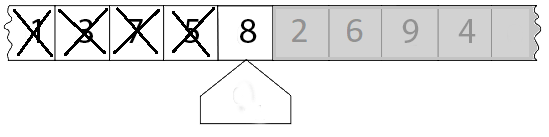
\includegraphics{slike/mat_formulacija.png}
    \caption{Izbira maksimalnega elementa zaporedja}
\end{figure}

Zanima nas \emph{najboljši način, s katerim je verjetnost, da je izbrani element maksimalen element niza, največja}.

Težava pri tej formulaciji je, da vemo, da je $N$ največji element naključne permutacije, in bi po zaporedju potovali, dokler ne bi prišli do elementa $N$. Vendar lahko v realnem življenju trenutno stanovanje le primerjamo s prejšnjimi s ``slabše'' ali ``boljše" in jim šele na koncu priredimo vsakemu svojo oceno.

%%%%%%%%%%%%%%%%%%%%%%%%%%%%%%%%%%%%%%%%%%%%%%
\section{Načini reševanja}

Zaradi lažjega razumevanja bomo v nadaljevanju namesto matematične uporabljali kar osnovno formulacijo s stanovanji. Sedaj iščemo način, ki maksimizira verjetnost, da bo izbrano stanovanje res najboljše od vseh.

Označimo z \textbf{$A$ dogodek, da izberemo najboljše stanovanje iz ponudbe $N$ stanovanj. Iščemo najvišjo verjetnost dogodka $A$}, torej najvišjo $P(A)$.

Zaradi lažjega računanja predpostavimo, da bi bile ocene stanovanj, če bi jih lahko vse ocenili, paroma različne. Najnižja ocena je 1, najvišja pa $N$. Torej imamo pred seboj \textbf{naključno permutacijo iz množice $S_{N}$}.

\subsection{Naključni izbor}

Ideja naključnega izbora je enostavna -- že pred začetkom ogledov se odločimo, katero stanovanje po vrsti bomo izbrali. S tem je verjetnost, da zadenemo najboljše stanovanje, enaka $P(A)=\frac{1}{N}$. To je hkrati tudi verjetnost, da izberemo kar prvo stanovanje in je le-to najboljše.
Vidimo, da z večanjem $N$ ta verjetnost pada proti 0, zato bi radi posikali kakšno boljšo rešitev (če obstaja).

\subsection{Reševanje z vzorcem}

Dozdeva se nam, da izbor naključnega stanovanja torej ni najboljša rešitev. Kaj lahko storimo? Ne ostane nam drugega, kot da si prvih nekaj stanovanj ogledamo.

Če še malo razmislimo, lahko pridemo do naslednje strategije: \textbf{ogledamo si prvih $K$ stanovanj} (to bo naš \emph{vzorec velikosti $K$}, kjer je $K$ omejen z $0 \leq K < N$), ki jih ocenimo, \textbf{a ne kupimo}. Potem pa nadaljujemo z ogledom in si \textbf{izberemo prvega, ki je boljše od najboljšega stanovanja iz vzorca} (glej \ref{NinvzorecK}).

\begin{figure}
    \centering
    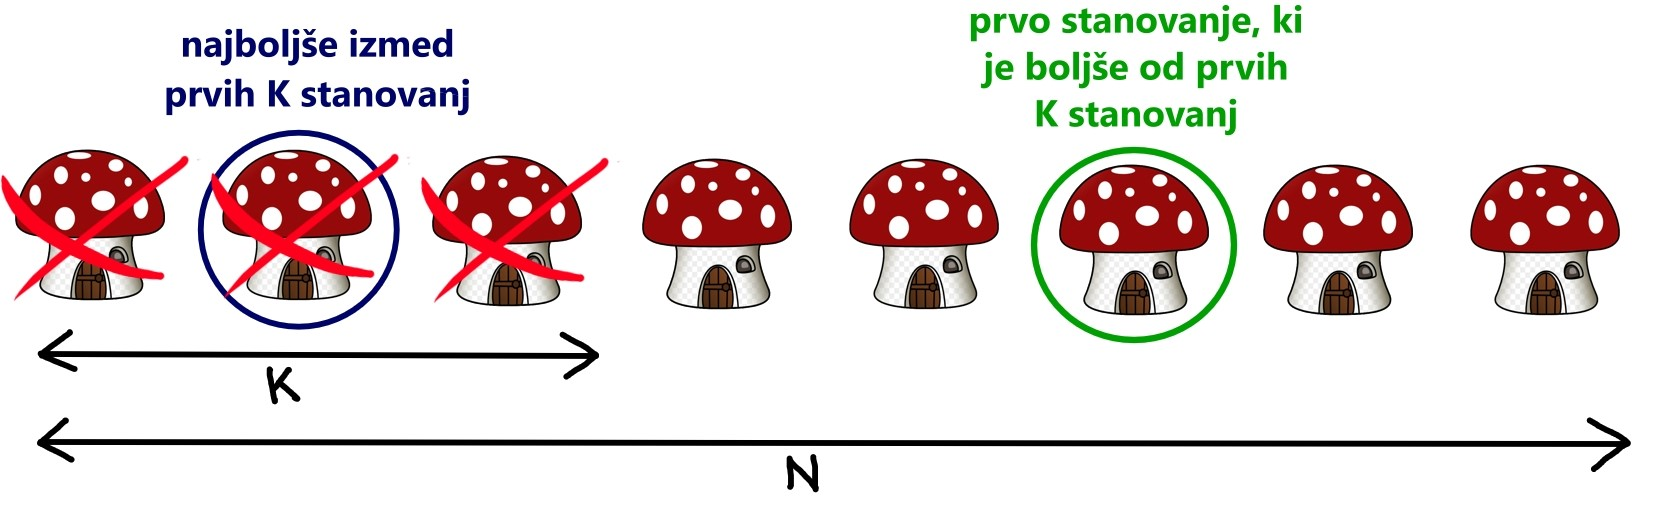
\includegraphics{slike/NinKformulacija2.jpg}
    \caption{Reševanje z vzorcem velikosti K}
    \label{NinvzorecK}
\end{figure}

V posebnem primeru $K=0$ si prej ne ogledamo nobenega stanovanja in kupimo prvo, torej je verjetnost uspeha enaka kot pri naključnem izboru, $P(A)=\frac{1}{N}$. V bistvu je naključna izbira poseben primer reševanja z vzorcem velikosti $0$. Če se zgodi, da se nam po $K$-tem stanovanju za nek $0 < K < N$ nobeno stanovanje ne zdi boljše, nam preostane zadnje, $N$-to stanovanje.

Poglejmo si najprej reševanje za majhne $N$, torej za majhno število stanovanj v ponudbi, za katere lahko ročno izračunamo želeno verjetnost. Kasneje pa bomo izračunali verjetnost za splošen, poljubno velik N.

\subsubsection{Reševanje za $N \in \{1,2,3,4\}$}

\subsubsection*{[$N=1$]}
Imamo eno stanovanje, ki je seveda najboljše, saj je edino v ponudbi. Torej $P(A)=1$ ne glede na način izbiranja. Vendar v primeru edine izbire ne vemo, kaj bomo dobili -- lahko je to stanovanje v odličnem stanju, lahko pa nam sploh ni všeč.

\subsubsection*{[$N=2$]}
Imamo dve stanovanji. Z naključnim izborom je $P(A)=\frac{1}{2}$. Če rešujemo z vzorcem, pa se verjetnost ne spremeni, saj imamo le dve možnosti -- ne ogledamo si nobenega in izberemo prvega ali pa si ogledamo prvega in izberemo drugega.

\subsubsection*{[$N=3$]}
Sedaj postane bolj zanimivo. Pred seboj imamo $3!=6$ permutacij ocen stanovanj. Če izberemo naključno stanovanje, je $P(A)=\frac{1}{3}$. Pri reševanju z vzorcem pa ločimo tri primere glede na število stanovanj v vzorcu, ki smo ga zgoraj označili s $K$.
\begin{itemize}
    \item $K=0$: Rešitev že vemo po naključnem izboru. Ogledamo si 0 stanovanj in izberemo prvega, ki je boljše, torej kar prvega. Sledi $P(A)=\frac{1}{3}$.
    \item $K=1$: Ogledamo si prvo stanovanje, a ga ne kupimo. Kupimo prvo, ki je boljše od prvega.

    Kot vidimo iz slike \ref{Nje3}, je $P(A)=\frac{3}{6}=\frac{1}{2}=50\%$.

    \item $K=2$: Ogledamo si prvi dve stanovanji in kupimo zadnje, zaradi simetrije je verjetnost enaka kot pri $K=0$, torej $P(A)=\frac{1}{3}$.
\end{itemize}

\begin{figure}
    \centering
    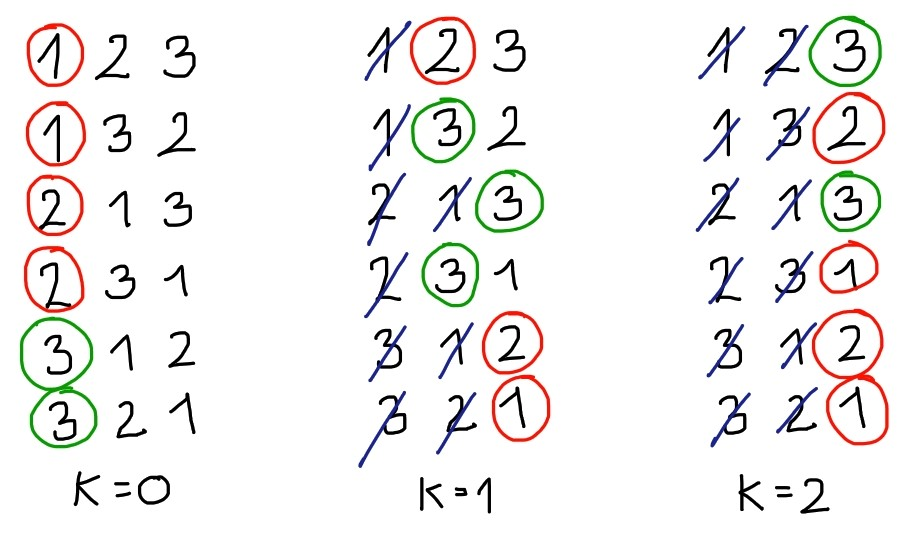
\includegraphics[scale=1.3]{slike/resevanje_N_3.jpg}
    \caption{Reševanje z vzorcem za tri stanovanja. Z zeleno so obkrožene uspešne izbire najboljšega stanovanja, z rdečo pa neuspešne izbire.}
    \label{Nje3}
\end{figure}

Zaključimo lahko, da se nam pri ponudbi treh stanovanj splača pogledati (vendar ne kupiti) prvo stanovanje ter izbrati prvega, ki je boljše od njega.

\subsubsection*{[$N=4$]}
Imamo $4!=24$ permutacij. Z naključnim izborom je $P(A)=\frac{1}{4}$. Poglejmo še rezultate izbiranja z vzorcem (računske korake spustimo, saj je postopek enak, vendar zaradi večjega števila permutacij daljši):
\begin{itemize}
    \item $K=0$: $P(A)=\frac{6}{24}=\frac{1}{4}$,
    \item $K=1$: $P(A)=\frac{11}{24}$,
    \item $K=2$: $P(A)=\frac{10}{24}$,
    \item $K=3$: $P(A)=\frac{6}{24}=\frac{1}{4}$.
\end{itemize}
Izkaže se, da je tudi pri štirih stanovanjih najbolje, da si ogledamo prvega in izberemo naslednjega boljšega.

\subsubsection{Rešitve za $N \in \{1,\ldots,10\}$}

Tudi za večje N se da po zgornjem postopku ročno izračunati verjetnost, vendar je časovno zamudno. Za $N \in \{1,\ldots,10\}$ so v tabeli \ref{tabela_z_verjetnostmi} zbrane verjetnosti glede na velikost $N$ in $K$. Za vsak $N$ je z modro označena najvišja verjetnost glede na $K$. S podatki iz tabel \ref{tabela_z_verjetnostmi} in \ref{tabela_z_verjetnostmi2} ter slike \ref{graf_delez_verjetnost} lahko sklepamo, da vzorec predstavlja približno prvo tretjino stanovanj, največja verjetnost pa se prav tako giba med 35--45\%.

\begin{table}[!ht]
    \centering
    \small
    \begin{tabular}[h]{|c|c|c|c|c|c|c|c|c|c|c|c|c|}
        \hline
        $K$ & $N=1$ & $N=2$ & $N=3$ & $N=4$ & $N=5$ & $N=6$ & $N=7$ & $N=8$ & $N=9$ & $N=10$ \\
        \hline
        0 & \cellcolor{blue!10}1 & \cellcolor{blue!10}0,5000 & 0,3333 & 0,2500 & 0,2000 & 0,1667 & 0,1429 & 0,1250 & 0,1111 & 0,1000 \\
        \hline
        1 & & \cellcolor{blue!10}0,5000 & \cellcolor{blue!10}0,5000 & \cellcolor{blue!10}0,4583 & 0,4167 & 0,3806 & 0,3500 & 0,3241 & 0,3020 & 0,2829 \\
        \hline
        2 & & & 0,3333 & 0,4167 & \cellcolor{blue!10}0,4333 & \cellcolor{blue!10}0,4278 & \cellcolor{blue!10}0,4143 & 0,3982 & 0,3817 & 0,3658 \\
        \hline
        3 & & & & 0,6667 & 0,3500 & 0,3917 & 0,4071 & \cellcolor{blue!10}0,4098 & \cellcolor{blue!10}0,4060 & \cellcolor{blue!10}0,3987 \\
        \hline
        4 & & & & & 0,2000 & 0,3000 & 0,3524 & 0,3798 & 0,3931 & 0,3982 \\
        \hline
        5 & & & & & & 0,1667 & 0,2619 & 0,3185 & 0,3525 & 0,3728 \\
        \hline
        6 & & & & & & & 0,1429 & 0,2321 & 0,2897 & 0,3274 \\
        \hline
        7 & & & & & & & & 0,1250 & 0,2083 & 0,2653 \\
        \hline
        8 & & & & & & & & & 0,1111 & 0,1889 \\
        \hline
        9 & & & & & & & & & & 0,1000 \\
        \hline
    \end{tabular}
    \caption{Verjetnosti, da izberemo najboljše stanovanje iz ponudbe $N$ stanovanj, kjer sta $N \in \{1,\ldots,10\}$ in $K \in \{0,\ldots,N-1\}$ velikost vzorca, zaokrožene na štiri decimalna mesta. Vzeto iz~\cite{secretary_puzzle}.}
    \label{tabela_z_verjetnostmi}
\end{table}

\begin{table}[!ht]
    \centering
    \small
    \begin{tabular}[h]{|c|c|c|c|}
        \hline $N$ & Najboljši $K$ & Delež $\frac{K}{N}$ & Maksimalen $P(A_{K})$ \\
        \hline 3 & 1 & 33,33\% & 50\% \\
        \hline 4 & 1 & 25,00\% & 48,53\% \\
        \hline 5 & 2 & 40,00\% & 43,33\% \\
        \hline 6 & 2 & 33,33\% & 42,78\% \\
        \hline 7 & 2 & 28,57\% & 41,43\% \\
        \hline 8 & 3 & 37,50\% & 40,98\% \\
        \hline 9 & 3 & 33,33\% & 40,60\% \\
        \hline 10 & 3 & 30,00\% & 39,87\% \\
        \hline 11 & 4 & 36,36\% & 39,84\% \\
        \hline 12 & 4 & 33,33\% & 39,55\% \\
        \hline 13 & 5 & 38,46\% & 39,23\% \\
        \hline 14 & 5 & 35,71\% & 39,17\% \\
        \hline 15 & 5 & 33,33\% & 38,94\% \\
        \hline 16 & 6 & 37,50\% & 38,81\% \\
        \hline 17 & 6 & 35,29\% & 38,73\% \\
        \hline 18 & 6 & 33,33\% & 38,54\% \\
        \hline 19 & 7 & 36,84\% & 38,50\% \\
        \hline 20 & 7 & 35,00\% & 38,42\% \\
        \hline
    \end{tabular}
    \caption{Optimalna izbira $K$ ter posledična delež stanovanj v vzorcu ter maksimalna verjetnost uspeha glede na število stanovanj $N \in \{3,\ldots,20\}$. Vzeto iz~\cite{secretary_puzzle}.}
    \label{tabela_z_verjetnostmi2}
\end{table}

\begin{figure}
    \centering
    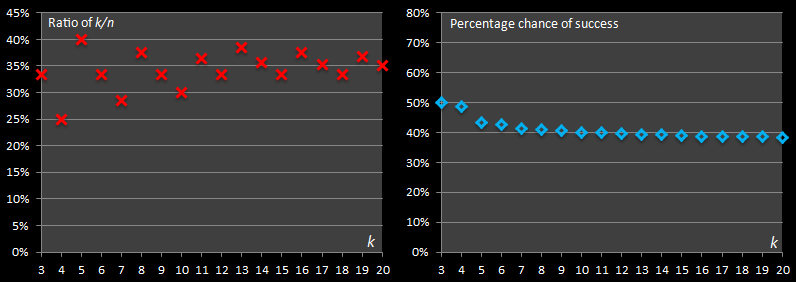
\includegraphics[scale=0.78]{slike/graf_delez_verjetnost.png}
    \caption{Sprememba deleža $\frac{K}{N}$ (levo) ter maksimalne verjetnosti (desno) z $N$. Vzeto iz~\cite{secretary_puzzle}.}
    \label{graf_delez_verjetnost}
\end{figure}

\subsubsection{Reševanje s splošnim $N$ in vzorcem velikosti $K$}

Rešimo problem še za splošen $N$ in $K$. Označimo s \textbf{$A_{K}$ dogodek, kjer preletimo prvih $K$ stanovanj, izberemo prvo, ki je boljše od vseh prejšnjih \emph{in} je le-to tudi najboljše stanovanje iz ponudbe}. Cilj naloge je \textbf{poiskati $K$} (oz. ekvivalentno delež stanovanj v vzorcu, torej $\frac{K}{N}$), \textbf{za katere je $P(A_{K})$ največja in koliko znaša.}

Za $K=0$ rezultat že vemo: ker izberemo kar prvo stanovanje, je $P(A_{0})=\frac{1}{N}$.

Opazimo lahko, da dogodek $A_{K}$ lahko zapišemu kot disjunktno unijo dogodkov glede na pozicijo najboljšega stanovanja v nizu:

\begin{equation*}
A_{K} = \bigcup^{N}_{n=1}\{\text{najboljše stanovanje je na poziciji $n$ IN izberem stanovanje na poziciji $n$}\}
\end{equation*}

Sedaj upoštevajmo tri stvari: \label{tristvari}
\begin{enumerate}
    \item tretji aksiom Kolmogorova: za paroma disjunktne dogodke $A_{1}, A_{2}, \ldots$ velja $$P(\bigcup^{\infty}_{n=1}A_{n}) = \sum^{\infty}_{n=1}P(A_{n}),$$
    \item prvih $K$ stanovanj ne moremo izbrati in
    \item formulo za pogojno verjetnost: $$P(A | B)=\frac{P(A \cap B)}{P(B)},$$
\end{enumerate}

iz česar sledi:

\begin{align*}
    P(A_{K}) &= \sum^{N}_{n=1}P(\text{izberem stanovanje na poziciji $n$} \cap \text{najboljše stanovanje je na poziciji $n$}) = \\
    &= \sum^{N}_{n=K+1}P(\text{izberem stanovanje na poziciji $n$} \cap \text{najboljše stanovanje je na poziciji $n$}) = \\
    &= \sum^{N}_{n=K+1}P(\text{najboljše stanovanje je na poziciji $n$}) \cdot \\
    & \qquad \qquad \cdot P(\text{izberem stanovanje na poziciji $n$ } | \text{ najboljše stanovanje je na poziciji $n$}).
\end{align*}

Vemo že, da je verjetnost, da najboljše stanovanje leži na neki poziciji, enaka $\frac{1}{N}$. Če predpostavimo, da najboljše stanovanje leži na poziciji $n$, pa ga lahko izberemo le, če se najboljše stanovanje med prvimi $n-1$ stanovanji nahaja v vzorcu, med prvimi $K$ stanovanji. Verjetnost tega dogodka pa je $\frac{K}{n-1}$. Dobimo

\begin{equation}\label{verezultatvsota}
    P(A_{K}) = \sum^{N}_{n=K+1} \frac{1}{N} \cdot \frac{K}{n-1}
    = \frac{1}{N} \sum^{N}_{n=K+1}\frac{K}{n-1}
    = \frac{K}{N} \sum^{N-1}_{n=K}\frac{1}{n}.
\end{equation}

\begin{wrapfigure}{R}{0.45\textwidth}
    \centering
    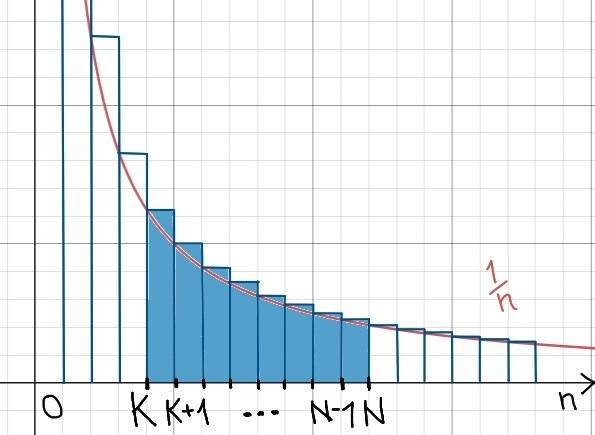
\includegraphics[scale=1.3]{slike/graf2.jpg}
    \caption{Delna Riemannva vsota funkcije $\frac{1}{n}$}
    \label{graf_1/n}
\end{wrapfigure}

Opazimo, da je vsota $\sum^{N-1}_{n=K}\frac{1}{n}$ delna Riemannova vsota za funkcijo $f(x)=\frac{1}{x}$ z delilnimi intervali dolžine $1$. Za male $N$ problem znamo rešiti, ko pa $N$ raste proti neskončnosti, ta vsota v limiti aproksimira ploščino pod grafom omenjene funkcije (glej sliko~\ref{graf_1/n}). Torej velja:

\begin{align*}
    \lim_{N \rightarrow \infty} P(A_{K}) &= \lim_{N \rightarrow \infty} \frac{K}{N} \int^N_{K}\frac{1}{x}dx = \\
    &= \lim_{N \rightarrow \infty} \frac{K}{N} \cdot \ln\frac{N}{K} = \\
    &= \lim_{N \rightarrow \infty} -(\frac{K}{N} \cdot \ln\frac{K}{N}).
\end{align*}

Označimo z $x = \lim_{N \rightarrow \infty} \frac{K}{N}$ in z upoštevanjem zveznosti funkcij za velike $N$ dobimo

\begin{equation}\label{priblizek_z_x}
    P(A_{K}) \approx - x \cdot \ln x.
\end{equation}

Zanima nas, za katere x bo ta verjetnost največja, kar zračunamo s pomočjo odvajanja:

\begin{align*}
    & P(A_{K})' = (- x \cdot \ln x.)' = - \ln x - 1 = 0 \\ & \Longrightarrow x = \frac{K}{N} = \frac{1}{e} \approx 37\% \Longleftrightarrow K = \frac{N}{e} \approx 0.37 N.
\end{align*}

Torej je najboljši vzorec tak, da zavrnemo prvih $\frac{N}{e}$ stanovanj in si izberemo prvega, ki je boljše od vseh prejšnjih. In verjetnost, da pri takšnem vzorcu zadenemo najboljše stanovanje, je ravno tako $P(A_{K}) = P(A_{\frac{N}{e}}) = - \frac{1}{e} \cdot \ln \frac{1}{e} = \frac{1}{e}$. Rezultat je ponazorjen tudi s grafom funkcije~\ref{priblizek_z_x} na sliki \ref{graf_xlnx}.

\begin{figure}[h]
    \centering
    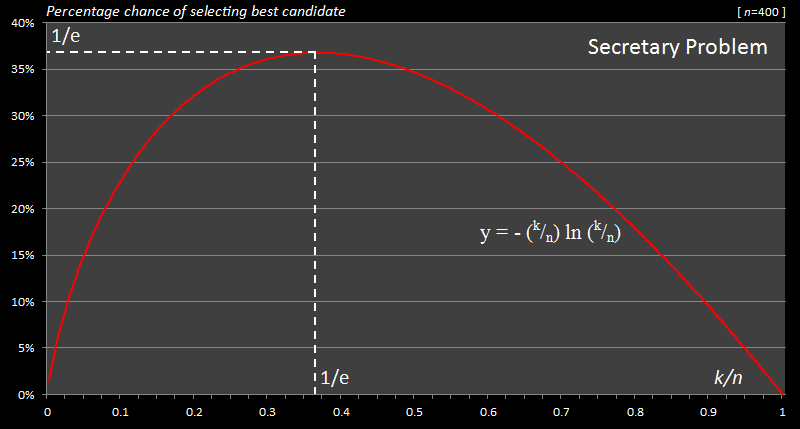
\includegraphics[scale=0.7]{slike/graf_xlnx.png}
    \caption{Možnosti izbire najboljšega stanovanja glede na delež stanovanj v vzorcu v procentih za $N = 400$. Vzeto iz~\cite{secretary_puzzle}.}
    \label{graf_xlnx}
\end{figure}

\newpage

%%%%%%%%%%%%%%%%%%%%%%%%%%%%%%%%%%%%%%%%%%%%%%
\section{Zaključek}

Osebno so mi najbolj všeč naloge, ki matematiko povezujejo s praktično uporabo in reševanjem problemov iz vsakdanjega življenja, zato je bilo ustvarjanje tega seminarja precej zanimivo. Če povzamem nalogo: Izmed N stanovanj, ki si jih ogledujemo vsakega posebej, moramo izbrati najboljšega, izbiramo pa lahko po vsakem ogledu, izbira o nakupu ali nenakupu pa se zgodi po vsakem ogledu, vse do izbire nakupa. Pri reševanju je bil najbolj pomemben razmislek, da si je potrebno prvih nekaj stanovanj ogledati ``za vzorec'' in glede na ta vzorec izbirati naprej, saj z naključno izbiro hitro pridemo do zelo majhne verjetnosti.

Za izbiranje s pomočjo postopka, kjer najprej pregledamo prvih nekaj stanovanj in kupimo prvega, ki je od njih boljše, je torej največja verjetnost uspeha, če najprej pregledamo prvih $\sim 37\%$ stanovanj. V tem primeru tudi verjetnost uspeha sama znaša $\sim 37\%$. Sicer rezultat ni najvišji, vendar nas po eni strani razveseli, saj je neodvisen od števila stanovanj v ponudbi.

Ta problem se da še razširiti na primer, ko bi bili kot kupec zadovoljni tudi s stanovanjem z nižjo oceno, vendar bi si vseeno postavili spodnjo mejo, npr. iz ponudbe z desetimi stanovanji bi bili zadovoljni s prvimi tremi. Reševanje tega primera se precej zaplete, vendar se v to nisem spuščala. Več na \cite{wikipedia_2022} in \cite{jstor_secretary_problem}.

%%%%%%%%%%%%%%%%%%%%%%%%%%%%%%%%%%%%%%%%%%%%%%
\newpage
\nocite{*}      % navede tudi vire, ki jih ne citiras
\printbibliography
%%%%%%%%%%%%%%%%%%%%%%%%%%%%%%%%%%%%%%%%%%%%%%
\end{document}